\section{Test requirements and proposed test  method}\label{sec:metrics}
%\hl{- What alternative method do we propose?}

The objective of the current tests is to validate the parameters of a well understood model of generation units. For the reasons given above, the new tests need to identify an empirical behavior model of an uncertain and diverse entity: the aggregator control architecture and unit portfolio. 

%This means that there is no single standard test, but 
A method is required to design the tests that will allow the system operators to understand and predict the performance of a specific aggregator under a given set of operation conditions (Fig.~\ref{fig:framework}). In this section we explain the underlying assumptions regarding the operating environment, the service requirement metrics used to measure the aggregator performance, and the proposed test design method.
%Getting an empirical model of an unknown entity rather than a mathematical model of a known entity. System identification approach.

\begin{figure}[!t]
\centering
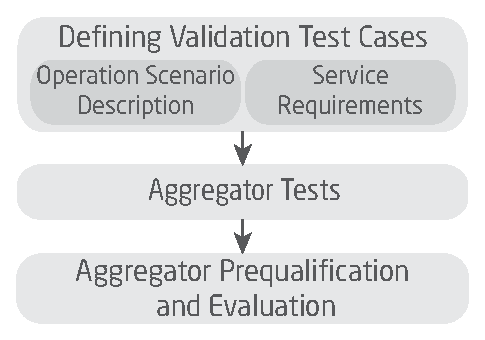
\includegraphics[width=1.7in]{pscc2016/validation.eps}
\caption{Schematic process for aggregator validation. The focus of this paper is on the relationship between the service requirements and the aggregator tests.}
\label{fig:framework}
\end{figure}

%Here the following three topics must be discussed:
%\begin{itemize}
%\item Boundary conditions (grid, DER)
%\item Fault scenarios
%\item Operation spectrum (what is the possibility/range of the input data?)
%\item Experimental design
%\end{itemize}

%The experiments should be able to measure response/states that can't be measured safely/easily under deployment.

%The tests must have a well defined input and output.

\subsection{Test environment assumptions}
The objective of the aggregator validation tests is to subject the aggregator to disturbances such that it can be verified that the aggregator is capable of respecting the service requirements under a set of expected operation scenarios. While the design of these operating scenarios is outside the scope of this paper, some overall assumptions can be made.

A great variety of aggregator architectures has been proposed and implemented; differences between them are linked to specific business cases, local regulations, grid codes etc. Implementation details such as algorithms for portfolio composition, resource prediction or trading, constitute key intellectual property of commercially operating aggregators and disclosure of these business secrets will be unacceptable in many cases. For this reason, a general test design must start from the assumption that the aggregator and its infrastructure are to be treated as a black box, in the sense that only the aggregator inputs and outputs are known but the details of the internal control architecture are unknown. 

While a few tests are enough to ensure compliance of traditional generators, the stochastic nature of aggregators requires the tests to be repeated a sufficient amount of times in order to capture the variance of the stochastic process that influences the aggregator performance. These stochastic processes, e.g. weather conditions or user behaviour, form the disturbances in the test. It is usually infeasible to subject a deployed and operational aggregator to a high number of tests, it is expected that aggregator validation must include simulation. In this way, the aggregator will be subjected to situations that are reproducible. It is assumed that such a simulation framework is detailed enough in terms of power system models, DER models and information and communication technology (ICT) systems in order for the simulation results to reflect the real performance of a deployed aggregator with sufficient precision.

The tests are composed of a set of operational scenarios and service requirements (Fig.~\ref{fig:framework}) wherein the operational scenarios define the statistical distribution of the test disturbances and the service requirements define the expected behavior of the aggregator. The mode of interaction between the test cases and the aggregator is defined in a test setup (Fig.~\ref{fig:test_setup}), where the disturbances (test inputs) defined in the operational scenarios affect the aggregator interaction with the DERs and the power grid. The aggregator has two interfaces:
\begin{itemize}
\item Input: Measurements or reference signals received from the system operators.
\item Output: Control domain signals and measurements exchanged between the aggregator and the units in its portfolio.
\end{itemize}

The operational scenarios are not designed to cover aggregator operation under exceptional system conditions. This means that the aggregator will not be held accountable for non-delivery in cases where the cause is outside of the aggregator's influence, e.g. in the case of grid faults. If communication between the aggregator and the controlled units, or internally within the aggregator architecture, occurs over public telecommunication networks, the robustness to network outages must be tested, for example by simulating disturbances and delays.

Finally, the flexibility which the aggregator can offer is bounded by the contractual requirements between the aggregator and its clients.

\begin{figure}[!t]
\centering
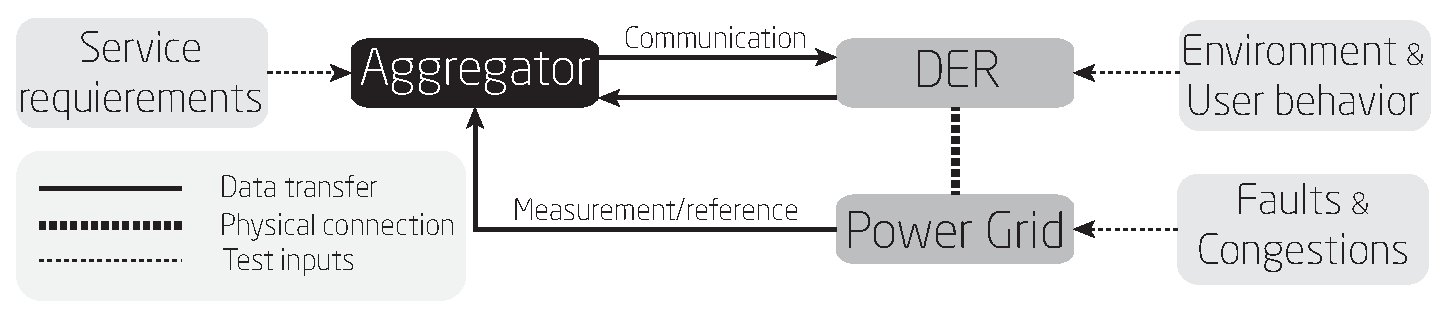
\includegraphics[width=\columnwidth]{pscc2016/test_setup.eps}
\caption{Schematic test setup where the test subject, the aggregator, is treated as a black box.}
\label{fig:test_setup}
\end{figure}

\subsection{Test service requirement metrics}\label{sec:servreqmet}

In order to measure how the disturbances affect service delivery, a set of service performance metrics must be established. The main purpose of the current tests is to verify communication, responsiveness to frequency changes and tracking of a reference or AGC\footnote{Automatic Generation Control, see e.g.\cite{entso1operational}.} signal. Coupling this with the performance requirements defined by the TSOs\fcite{energinettender,ipower2013development}, the expected behavior of the considered services was analyzed (Table~\ref{tab:servmet}), and a set of requirement metrics were defined:
\begin{itemize}
\item Time responsiveness, i.e. how fast can the service be delivered from the moment the reference or measurement signal changes.
\item Grid responsiveness, i.e. how well can the aggregator follow changes in the grid state (marked with $\star$ where relevant on Tab.~\ref{tab:servmet}).
\item Response accuracy, i.e. how good is the aggregator in providing the full volume that is requested.
\end{itemize}


\begin{table}[!t]%% increase table row spacing, adjust to taste
\renewcommand{\arraystretch}{1.3}
% if using array.sty, it might be a good idea to tweak the value of
% \extrarowheight as needed to properly center the text within the cells
\caption{System services and their behavior}
\label{tab:servmet}
\centering
% Some packages, such as MDW tools, offer better commands for making tables
% than the plain LaTeX2e tabular which is used here.
\begin{tabularx}{\columnwidth}{p{1.0cm} X X}
\toprule
System Operator& Service name & Service behavior\\
\midrule
TSO & Frequency containment reserve (FCR) & autonomous response to frequency deviations ($\star$) \\
TSO & Frequency restoration reserve (FRR) & tracking of the AGC-signal\\
DSO & Congestion management         & reference tracking \\
    &                               & respecting a maximum feeder/transformer limit ($\star$) \\
    &                               & demand response \\
    &                               & grid state responsiveness ($\star$)\\
\bottomrule
\end{tabularx}
\end{table}

These three metrics will conform the measure with which an aggregator will be deemed to perform according to service requirements, and the tests must excite the aggregator such that it is possible to determine through the value of these metrics the performance of the aggregator. It must be pointed out that the grid responsiveness metric is only applicable to the evaluation of aggregators providing services that rely on direct measurement of the grid, e.g. FCR.

It is assumed that the validation tests will be carried out in simulation so that the tests can capture the stochastic nature of the disturbances. Therefore, when system operators define the acceptable values of the service requirement metrics, the values should have a statistical component. An example could be that the time responsiveness of a service provision should in average of 5 seconds, with a variance of $\pm$ 1 second. The actual indices used for the proposed metrics are discussed in Sec.\ref{sec:evaluation}.

\subsection{Aligning service requirements and tests}\label{sec:alignment}
In order to align the service requirements and the test design, we propose the following steps:
\begin{enumerate}
	\item The aggregator informs of the general composition of its portfolio, as well as the service it wants to be validated for.
	\item The tester identifies the appropriate service requirements for the service to be tested for.
	\item The tester identifies the expected normal operation of the aggregator.
	\item The tester defines the operation scenarios that the aggregator is expected to perform under. The scenarios must define the statistical properties, e.g. mean and variance, for the stochastic disturbances affecting the aggregator performance.
	\item The tests are carried out on the aggregator.
	\item The aggregator performance is evaluated.
\end{enumerate}

From the services analysed in this work, we divide the tests into two categories depending on their excitation signal:
\begin{itemize}
\item step response (like those for FCR),
\item continuous reference tracking (like those for FRR).
\end{itemize}

The validation tests will use one of these excitation signals under a different set of circumstances defined in the operation scenarios. The same excitation signal will be applied to the aggregator a sufficient amount of times to ensure that the mean and variance of the performance metrics give a realistic impression of the aggregator performance under deployment.%Thus, we formulate the following heuristic for the alignment of service requirements and tests: if a service
%The tests will evaluate the sensitivity of the aggregator to changes in the portfolio, and issues with the communication.

A drawback of this method, in comparison with the traditional test method, is that the overall validation method rely on the accuracy of the simulation models. The test architecture that validates the aggregators itself would need to be validated. This applies to the communication systems, the grid models and the DER models.

%\hl{The test procedure should be described. 2 diagrams are needed: 1st. shows the aggregator under normal operation (physical connection and the ICT connection), with relevant inputs and outputs of the aggregator. 2nd is the test process, where at each stage inputs are added/modified.}

% At the same time, based upon these two inputs, the overall service delivery is verified and evaluated, which is reflected in the bottom box of Figure~\ref{fig:framework}. \hl{Generally, I think we're still talking too much about the overall process and not about what the paper claims it's focusing on ("[...] the alignment of service requirements with the testing [...]"). On the latter we're not specific enough wrt what kind of result the reader can expect.}

%An aggregator infrastructure and control process is usually complex and therefore interactions of an aggregator may be tested separately. Depending on the metrics by which the relations are measured (Table~\ref{tab:metrics}), it is possible to test certain components through simulation or co-simulation, while other interactions require hardware-in-the-loop tests. This paper will propose a method for identifying the relationships between metric types and the tests necessary  for validating the measured function. The method will then be applied to several existing aggregator architectures as a proof of concept.

\subsection{Test evaluation}\label{sec:evaluation}
The service requirement metrics (Sec.~\ref{sec:servreqmet}) define the measure upon which the aggregator is evaluated. Different options exist that can be used to measure these metrics. One option is the aggregator performance index\fcite{bondy2014performance}, which measures the error in service delivery for the services delivered to the system operators and the serviced delivered to the owners of the DERs. This metric captures both time responsiveness and response accuracy into a single value. A large set of performance indices exist within the field of control performance assessment, these can be utilised for the proposed validation method\fcite{Jelali}.

Given the stochastic nature of the tests, the indices will also be stochastic. The value of the performance indices is estimated at each iteration of the test, which means that the final value of the performance index reflects the stochasticity of the disturbances. For example, if the disturbances defined in the operation scenarios are Gaussian, the performance index will also have a mean and variance. These values need to be compared to those values defined in the service requirements. It will be the choice of the system operators what the service requirements should be, taking into consideration their risk adversity. Requiring a small variance on the performance indices minimizes the risk of not getting a full service delivery, but might also lead to more expensive services.

